\section{Mistery Scheduler}

A partir del \texttt{.o} de un scheduler, hicimos ingeniería inversa de su comportamiento a partir de la ejecución de varias instancias.

\subsection{Analisis}

Para tener una idea de lo que hace el scheduler probamos con los siguientes parametros:

\begin{enumerate}
	\item lote\_tsk: 2.tsk
	\item num\_cores: 1
	\item switch\_cost: 0
	\item sched\_class: SchedFCFS
	\item params: 5 6 7 8 9 10
\end{enumerate}

Primero ejecutamos las siguientes tareas

\begin{itemize}
	\item Tarea 0: 90 ciclos de CPU, 0 llamadas bloqueantes
	\item Tarea 1: 90 ciclos de CPU, 0 llamadas bloqueantes
	\item Tarea 2: 90 ciclos de CPU, 0 llamadas bloqueantes
\end{itemize}

El resultado fue el siguiente:

\begin{figure}[h]
    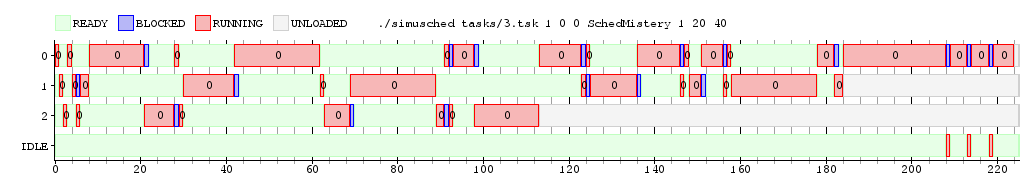
\includegraphics[width=\linewidth]{images/mist.png}
    \label{fig:Task Consola}
    \caption{Primera prueba}
\end{figure}

Aqui podemos apreciar que el scheduler tiene una cierta similitud con $Round Robin$, donde el quantum varia de manera rotativa segun los parametros pasados al scheduler. La primera vez que el proceso ejecuta lo hace por un ciclo y es desalojado, luego el quantum es determinado por los parametros recibidos hasta llegar al ultimo, a partir de ese momento el quantum es siempre el mismo hasta que el proceso termina de ejecutarse.

\pagebreak

Con esto en mente, procedimos a ver como operaba el scheduler con la incorporacion de tareas. Para esto se ejecutaron las siguientes tareas:

\begin{itemize}
	\item Tarea 0: 90 ciclos de CPU, 2 llamadas bloqueantes, incorporada en el momento 0
	\item Tarea 1: 90 ciclos de CPU, 4 llamadas bloqueantes, incorporada en el momento 20
	\item Tarea 2: 90 ciclos de CPU, 6 llamadas bloqueantes, incorporada en el momento 40
\end{itemize}

\begin{figure}[h]
    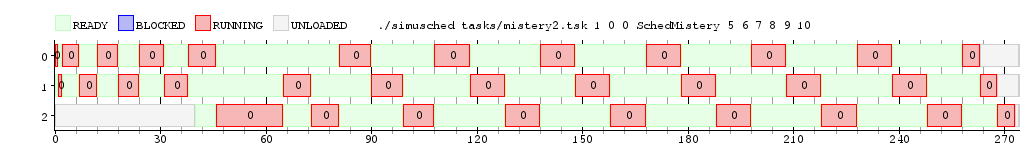
\includegraphics[width=\linewidth]{images/mist2.png}
    \label{fig:Task Consola}
    \caption{Segunda prueba}
\end{figure}

En este caso, al incorporar la tarea podemos observar que su quantum asignado es sumamente grande. Luego de mucho análisis observamos que en realidad estaba sumando los quantums que habíamos pasado por parámetro. Aquí es donde nos dimos cuenta que probablemente el Scheduler tenia múltiples colas con diferentes prioridades dadas por los parámetros de entrada. Siempre se ejecuta la tarea de máxima prioridad. La tarea 2 en un inicio se ejecuta por un quantum grande dado que se le suma el quantum de las colas de prioridad 1, 5, 6 y 7.

\hspace{1px}

Finalmente, buscamos ver como funcionaba el scheduler al incorporarse una tarea bloqueante.

\begin{figure}[h]
    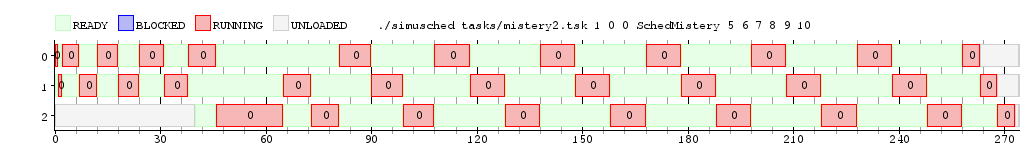
\includegraphics[width=\linewidth]{images/mist2.png}
    \label{fig:Task Consola}
    \caption{Tercera prueba \textbf{PONER LA POSTA}}
\end{figure}

Notamos que al entrar una tarea bloqueante seguía ejecutando la próxima de la cola y continuaba el Round Robin. Sin embargo, también notamos que al reincorporarse la tarea la misma tenia el quantum correspondiente a una cola con exactamente un nivel mayor de prioridad. De esta manera inferimos que al momento de reincorporar una tarea el scheduler si puede la asigna a una cola con un nivel mas de prioridad. A su vez, esto significa que en muchos casos esta sera la primera en ejecutarse al reincorporarse, sin tener que esperar al resto de las tareas que ya estaban en ejecución.

\hspace{1px}

Para concluir, el Mystery Scheduler es un scheduler con Round Robin y múltiples colas de prioridad. A cada cola de prioridad se le asigna un quantum único dado por parámetro. Existe una cola implícita, que es la de mayor prioridad, con un quantum de 1. Cada cola adicional que se agrega tiene el quantum pasado por parámetro pero una prioridad menor. El scheduler siempre busca nuevas tareas en las colas de mayor prioridad. Si no encuentra una tarea en dicha cola, pasa a la siguiente.  Al bloquearse una tarea, la misma se remueve del scheduler y luego se reincorpora agregándose a una cola de tareas con un nivel de prioridad mayor. Tener una prioridad mayor no necesariamente implica tener un quantum mayor asignado, solo que se la ejecutara primero.

\pagebreak

\subsection{Código}

\subsubsection{Class Declaration}
\begin{lstlisting}[language=C++, breaklines=true]
class SchedNoMistery : public SchedBase {
  public:
    SchedNoMistery(std::vector<int> argn);
    virtual void load(int pid);
    virtual void unblock(int pid);
    virtual int tick(int cpu, const enum Motivo m);
  private:
	std::vector<int> quantum_list;
	std::vector<std::queue<int> > q;
  std::map<int, int> blockedQueue;
	int cycles_left, current_queue, tasks;
	int next_pid(void);
};
\end{lstlisting}


\subsubsection{Constructor}
\begin{lstlisting}[language=C++, breaklines=true]
SchedNoMistery::SchedNoMistery(vector<int> argn) {
	// cpu cores, rest of params
	cycles_left = 1;
	current_queue = 0;
	tasks = 0;

	quantum_list.push_back(1);
	q.push_back(queue<int>());

	if (argn.size() > 1) {
		for (vector<int>::iterator it = ++argn.begin(); it != argn.end(); ++it) {
			quantum_list.push_back(*it);
			q.push_back(queue<int>());
		}
	}
}
\end{lstlisting}


\subsubsection{Load y Unblock}
\begin{lstlisting}[language=C++, breaklines=true]
void SchedNoMistery::load(int pid) {
	q.at(0).push(pid);
	tasks++;
}
\end{lstlisting}

\begin{lstlisting}[language=C++, breaklines=true]
void SchedNoMistery::unblock(int pid) {
	q.at(max(0,blockedQueue[pid]-1)).push(pid);
	blockedQueue.erase(pid);
	tasks++;
}
\end{lstlisting}


\subsubsection{Tick}
\begin{lstlisting}[language=C++, breaklines=true]
int SchedNoMistery::tick(int cpu, const enum Motivo m) {
	if (m == EXIT || m == BLOCK) {
		if (m == BLOCK) {
			blockedQueue[current_pid(cpu)] = current_queue;
		}
		
		tasks--;
		// current pid ended, get next
		if (tasks == 0) return IDLE_TASK;
		else { // get task from list
			return next_pid();
		}
	} else {
		if (current_pid(cpu) == IDLE_TASK && tasks > 0) {
			return next_pid();
		} else {
			cycles_left--;
			if (current_pid(cpu) != IDLE_TASK && cycles_left == 0) {

				current_queue = min(current_queue + 1, ((int) q.size()) - 1);
				if (tasks == 0) {
					cycles_left = quantum_list.at(current_queue);
					return current_pid(cpu);
				} else {
					q.at(current_queue).push(current_pid(cpu));
					return next_pid();
				}
			}
			return current_pid(cpu);
		}
	}
}

/* Requires some queue not to be empty */
int SchedNoMistery::next_pid() {
	int selectQueue = 0;
	for (vector<queue<int> >::iterator it = q.begin(); it != q.end(); ++it) {
		if ((*it).size() > 0) break;
		selectQueue++;
	}
	int pid = q.at(selectQueue).front();
	q.at(selectQueue).pop();
	current_queue = selectQueue;
	cycles_left = quantum_list.at(selectQueue);
	return pid;
}

\end{lstlisting}

\pagebreak

\textbf{BORRAR LO SIGUIENTE?}

\subsection{Diagramas y analisis del scheduler}
Para poder analizar el comportamiento del scheduler, decidimos armar el siguiente lote de tareas:

\begin{lstlisting}
	*3 TaskCPU 10
@4
*3 TaskCPU 5

TaskConsola 2 1 4
TaskConsola 5 1 1
TaskConsola 10 1 2
*3 TaskCPU 10
@20:
TaskCPU 10
\end{lstlisting}

De este gráfico podemos inferir lo siguiente:

\begin{itemize}
	\item El scheduler es un round robin con algunas particularidades
	\item Al incoporarse una nueva tarea, se la coloca en el tope de la cola del scheduler.
\end{itemize}

Este ultimo punto es importante, si dos tareas se incoporan durante la ejecucion de otra tarea, primero concluye el quantum de la tarea actual y se procede a cambiar la tarea con la primera que llego. Es por esta razon que elegimos implementar el scheduler sobre una lista, ya que nos permite agregar los elementos en las posiciones que precisamos.

Otra cosa que determinamos mediante experimentacion, es que el scheduler toma una cantidad arbitraria de parametros. Despues de varias pruebas, pudimos determinar el comportamiento del scheduler respecto a los parametros. Si tomamos los parametros \texttt{5 4 3 2 1}, todas las tareas van a ejecutarse por primera vez con un quantum de un ciclo (esto es independiente de los parametros). Posteriormente el scheduler toma los valores del quantum a partir de los parametros del scheduler de forma ordenada y ciclica, es decir, el quantum de una tarea seria \texttt{1}, \texttt{5}, \texttt{4}, \texttt{3} ,\texttt{2}, \texttt{1}, \texttt{5}, \texttt{4} y asi sucesivamente hasta que concluye la ejecucion de la tarea.

Por ultimo, esta el analisis como responde el scheduler ante las llamadas bloqueantes. Si una tarea tiene una llamada bloqueante se procede a desalojarla hasta que la misma se resuelve, una vez que se resuelve se procede a agregarla nuevamente a la lista con un quantum de un ciclo. Esto ocurre independientemente de los parametros que recibe el scheduler.